\section*{Appendix: Injected Potential for \( m = 12 \)}
\vspace{5pt}
Computed with \( t = 0.1 \), normalized \( \psi_0 \):
\[
V_{\text{mod}} = \begin{bmatrix}
1.697506, & 1.463694, & 1.704297, & 1.706590, & 1.704297, & 1.463694, \\
1.697506, & 1.463694, & 1.704297, & 1.706590, & 1.704297, & 1.463694
\end{bmatrix}.
\]

\begin{figure}[h]
\centering
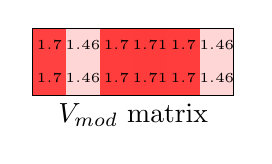
\begin{tikzpicture}[scale=0.85]
    % Visualize the matrix structure of V_mod
    \foreach \x/\v in {0/1.697506, 1/1.463694, 2/1.704297, 3/1.706590, 4/1.704297, 5/1.463694, 6/1.697506, 7/1.463694, 8/1.704297, 9/1.706590, 10/1.704297, 11/1.463694} {
        \pgfmathsetmacro{\cell}{int(\x/6)}
        \pgfmathsetmacro{\idx}{\x-\cell*6}
        \pgfmathsetmacro{\intensity}{100*(\v-1.4)/0.4}
        \fill[red!\intensity] (\idx*0.5,\cell*0.5) rectangle (\idx*0.5+0.5,\cell*0.5+0.5);
        \node at (\idx*0.5+0.25,\cell*0.5+0.25) {\tiny \pgfmathprintnumber[fixed, precision=2]{\v}};
    }
    
    % Add a border
    \draw (0,0) rectangle (3,1);
    
    % Title
    \node at (1.5,-0.3) {$V_{\text{mod}}$ matrix};
\end{tikzpicture}
\caption{Heat map visualization of the $V_{\text{mod}}$ matrix for $m=12$, showing the pattern of lower potential values in prime-rich residue classes.}
\label{fig:vmod_matrix}
\end{figure}